% -*- mode: LaTeX; coding: utf-8; -*-

% Artikkelia varten.
\ifdefined\seminaari
\begin{abstract}
\else
\chapter{Web-palvelut ja niiden tietoturva}
\fi

Toimivan ja turvallisen Web-pohjaisen palvelun tarjoaminen vaatii
nykyisin todella paljon aikaa ja huolellisuutta sekä palvelun kehittäjältä että
palvelun tarjoajalta ja ylläpitäjältä. Ajat ovat muuttuneet siitä,
jolloin käyttäjät selailivat pääasiassa staattisia Web-sivuja, ja käyttivät tarjotuista
palveluista korkeintaan sähköpostia. Kehitys kulkee kovaa vauhtia eteenpäin, ja
tämän päivän suurimpia trendejä ovat interaktiivisuus, sosiaalisuus ja yksilöllisyys, 
joiden avustuksella verkon käytöstä on pyritty tekemään
käyttäjille entistä henkilökohtaisempi kokemus. Palvelut kuten MySpace,
Facebook ja YouTube ovat vahvistaneet näitä käyttäjätottumuksia, ja
markkinoille on syntynyt kova kilpailu siitä, kuka kehittää seuraavan
menestyspalvelun. Nykyisin puhutaankin Internetin seuraavasta evoluutiosta Web 2.0:n 
muodossa, joita myös edellä mainitut palvelut edustavat. Uudet teknologiat ja
kiire tuovat kuitenkin aina mukanaan joukon uusia heikkouksia, joita hyökkääjät
pyrkivät hyödyntämään. 

\ifdefined\seminaari
\end{abstract}
\license
\pagebreak
\else
\relax
\fi

\section{Dynaaminen Web}

Web 2.0 on termi, jota käytetään monessa eri merkityksessä ja
asiayhteydessä. Se yhdistetään usein uusiin dynaamisiin Web-\-teknologioihin ja In\-ter\-net-
ai\-ka\-kau\-den tuotteiden ja palveluiden kehityskaarien kuvaamiseen \cite{WEB2}. Yhteistä näille
on se, että ne pyrkivät esittämään sitä muutosta ja kasvua, jota Internet pitää tällä
hetkellä sisällään. Tämä muutos on lähtöisin siitä, että kuluttajatottumukset
ovat kehittyneet kohti interaktiivisia palvelumalleja, joissa käyttäjillä on
entistä suurempi mahdollisuus vaikuttaa siihen, miten haluttu informaatio esitetään.
Sosiaalisuus ja sen luoma yhteisöllisyys ovat luoneet tarpeen palveluille,
joissa käyttäjät pystyvät tekemään useita asioita saman aikaisesti saumattomasti
yhdestä paikasta käsin. Toinen kantava voima  muutokselle on ollut markkinoiden
tuoma paine, johon yritykset ovat pyrkineet mukautumaan sekä kuluttaja- että yrityspuolella. 
Tätä varten yritykset ovat kehittäneet entistä suurempia ja 
monimutkaisempia palvelukokonaisuuksia uusilla teknologioilla, joiden käyttöä ei aina riittävästi hallita. 
Tähän kun lisätään kiire päästä markkinoilla ensimmäisten
joukossa, niin tietoturva-asiat jäävät usein taka-alalle \cite{WEB2b}.

Tietoturvan kannalta teknologiat, jotka luetaan kuuluvan osaksi Web 2.0
teknologiaperhettä, ovat jatkuvan huomion ja kehityksen kohteena. Nämä teknologiat
muodostavat sen voiman, joka mahdollistaa siirtymisen dynaamisiin
sovelluksiin, kuten Google Maps ja yritysten toimintojen ohjaamisen verkkoon.
Teknologiat kuten Asynchronous JavaScript And XML (AJAX), Cascading Style Sheet (CSS),
Flash, JSON ja XML voidaan kaikki laskea kuuluvan osaksi Web 2.0-perhettä.
Osa näistä teknologioista on ollut jo pidemmän aikaa käytössä, kun taas osaa on
vasta nyt alettu hyödyntämään siihen, mihin ne on alun perin suunniteltu \cite{WEB2}.
Kuvassa \ref{web} on nähtävillä näiden yleisimpien teknologioiden ja protokollien
väliset suhteet.

\begin{figure}[htp]
\centering
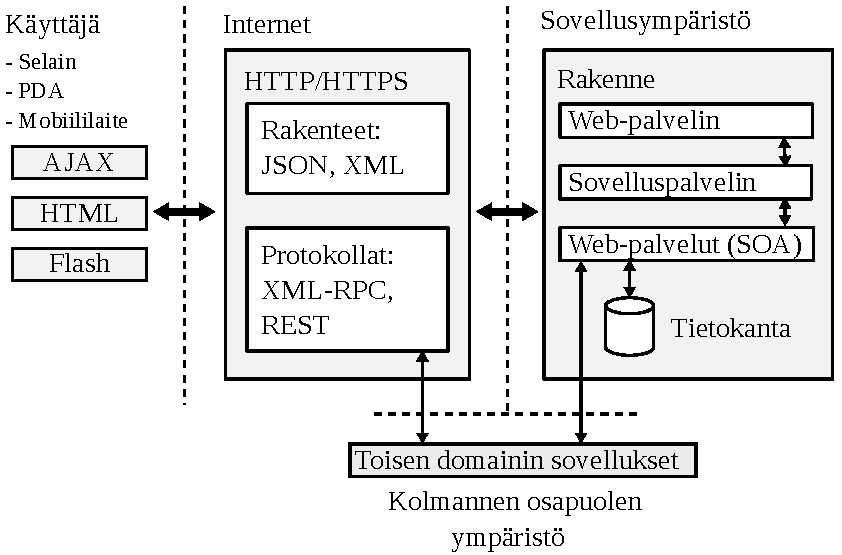
\includegraphics[width=12cm]{pics/web_ymparisto.pdf}
\caption{Web 2.0 -teknologiaperhe.}
\label{web}
\end{figure}

Tietoturvan kannalta dynaamiset Web-teknologiat tuovat mukanaan joukon uu\-si\-a haasteita. Ensinnäkin
samat vanhat tietoturvariskit, jotka vaivasivat jo Web 1.0 aikoihin, ovat edelleen voimassa. Näiden lisäksi
hyökkäykset kuten Cross-Site Scripting (XSS) ja Cross-Site Request Forgery (CSRF) 
ovat aikaisempaa vaarallisempia, koska käytetyt teknologiat tarjoavat
monipuolisemman ympäristön, jonka kautta murtautua järjestelmiin \cite{WEB2}. Dynaamiset
Web-sovellukset antavat myös loppukäyttäjille ja takana oleville ohjelmille enemmän
valtaa, jonka johdosta loppukäyttäjä ei välttämättä edes huomaa joutuessaan
tietomurron kohteeksi. Tästä hyvänä esimerkkinä Ajax-teknologia, joka mahdollistaa
sivujen tietojen päivittämisen käyttäen asynkronisia kutsuja. Tekniikan ansiosta
käyttäjä pystyy tekemään kutsuja palvelimille ja päivittämään osan sivun
tiedoista niin, ettei koko sivua tarvitse päivittää. Tästä suurin osa tapahtuu
käyttäjältä piilossa, joten hän ei todennäköisesti huomaa, jos selain lataa
haitallisia skriptejä koneelle käyttäen jotain tunnettua tietoturva-aukkoa. Yhden
arvion mukaan jopa 70 prosenttia kaikista haitallisista koodeista ladataankin käyttäen
Ajaxia \cite{WEB2c}.

Palvelinpuolella muutokset eivät rajoitu vain dynaamisten Web-\-teknologioiden tuomiin
tietoturvariskeihin, sillä uudenlainen ajattelu vaatii myös uudenlaista
palveluarkkitehtuuria. Uusi arkkitehtuuriratkaisu tuo aina mukanaan suuren
joukon muutoksia, jotka tulee ottaa huomioon tietoturvan suunnittelussa.
Palvelukeskeinen arkkitehtuuri (engl. Service Ori\-ent\-ed Architecture, SOA) on
yksi näistä kehysmalleista, joka on kasvattanut suosiotaan Web 2.0:n
vanavedessä. SOA-ark\-ki\-teh\-tuu\-ril\-la onkin nykyisin tärkeä rooli palvelujen
välisen kommunikoinnin kehittämisessä. Siksi on tärkeää ymmärtää, mistä
palasista SOA-arkkitehtuuriin perustuvat palvelut koostuvat, ja mitä tämä
merkitsee tietoturvan kannalta.

\section{Palvelukeskeinen arkkitehtuuri}

Web-pohjaiset sovellukset ovat saaneet yhä suurempaa huomiota yritysten
tuotekehityksessä. Muutoksen taustalla on teknologian
kehittyminen siihen pisteeseen, missä toimittajat pystyvät
luotettavasti ja nopeasti tarjoamaan aikaisempien
palvelin-asiakas -sovelluksien sijaan verkon välityksellä käytettäviä sovelluksia. Tämä
ratkaisu on tuonut mukanaan taloudellisia säästöjä yrityksille, jotka ovat ennen
joutuneet itse huolehtimaan muun muassa sovellusten ajan tasalla pitämisestä ja
palvelimien ylläpitämisestä \cite{WEB2}. Muutos on luonut myös tarpeen löytää yhä
tehokkaampia kehitysmalleja ja tapoja toteuttaa entistä monimutkaisempia ja
vaativimpia sovelluksia suuryritysten tarpeisiin. Yksi tapa hallita tätä
muutosta on perustaa tehdyt ohjelmistosuunnittelun ratkaisut palvelukeskeisen
arkkitehtuurin malliin.

Puhuttaessa dynaamisista Web-palveluista, palvelukeskeinen arkkitehtuuri lähtee siitä
ajatuksesta, että palveluiden toiminnot ja prosessit pyritään suunnittelemaan
toimimaan mahdollisimman itsenäisesti ja avoimesti siten, että niitä pystytään
kutsumaan joustavasti eri sovellusten välillä käyttäen standardoitua rajapintaa.
Tähän ratkaisuun ovat ajaneet pyrkimys laskea IT-kustannuksia ja
uudelleenkäytön maksimointi jo käytössä olevissa 
ratkaisuissa. Aikaisemmin tämän toteuttaminen
on ollut vaikeaa sovellusten heterogeenisyyden takia, jolloin eri
alustojen ja toimittajien väliset yhteistoiminnot ovat olleet usein mahdottomia
toteuttaa. Yhä useamman sovelluksen ja palvelun siirtyessä verkkoon tästä
rajoitteesta pyritään nyt pääsemään eroon, ja tähän ongelmaan palvelukeskeinen arkkitehtuuri
on suunniteltu tuomaan ratkaisu.

Käytännössä siirtyminen palvelukeskeiseen arkkitehtuuriin tarkoittaa sitä, että arkkitehtuurin
tulee tarjota sovelluksille mahdollisimman joustava sekä sijainnista ja
protokollasta riippumattoman alusta \cite{SOA}. Tämän avulla loppukäyttäjälle
voidaan tarjota palveluita monesta eri paikasta yhtä aikaa siten, ettei hän ole
edes tästä tietoinen. Kyseessä on sama ajattelumalli, johon dynaamiset Web-sovellukset
pohjautuvat, ja siksi palvelukeskeinen arkkitehtuuri on saanut paljon
nostetta Web 2.0:n myötä.

Palvelukeskeisen arkkitehtuurin tuomat edut eivät rajoitu pelkästään
kustannussäästöihin. Sen tuomiin etuihin kuuluu myös muun muassa uu\-si\-en toimintojen
helpompi integrointi jo käytössä oleviin järjestelmiin sekä monimutkaisten
kokonaisuuksien sujuvampi hallinta. Organisaatioille on myös tärkeää, että tällä
tavalla suunniteltuihin palvelumalleihin on nopeampi tehdä haluttuja muutoksia, jolloin 
reagointi markkinamuutoksiin voidaan toteuttaa nopeassa aikataulussa \cite{WEB2c}. Tämä on
erityisen tärkeää, koska markkinoille on ilmestynyt monia uusia tekniikoita,
jotka mahdollistavat Web-palveluiden integroinnin jo käytössä oleviin
palveluihin.

Vuonna 2008 Web-pohjaisten palveluiden kehittämiseen
käytettiin arviolta yli 11 miljardia dollaria ja osa fokuksesta on jo siirtynyt
kohti keskikokoisia ja pieniä yrityksiä. Web-pohjaisten palveluiden merkityksen
uskotaan entisestään kasvavan ja yritykset, jotka reagoivat hitaasti tähän
muutokseen, huomaavat tulevaisuudessa olevansa epäsuotuisassa asemassa \cite{WEB2b}.

Palvelimen arkkitehtuurissa tapahtuvat muutokset tarkoittavat sopeutumista uudenlaiseen
ajattelumalliin, jossa palvelut on hajautettu ympäri verkkoa. Näistä palveluista kaikki
eivät välttämättä ole yhteisen tietohallinnon alaisuudessa. Kuvan \ref{soa} mukainen ratkaisu
tulee olemaan tulevaisuudessa arkipäivää ja se tuo mukanaan uusia rajapintoja,
joiden kautta hyökkääjä voi pyrkiä murtautumaan järjestelmään tai jopa
yrityksen sisäiseen verkkoon. Koska palveluiden välinen kommunikointi perustuu
tässä mallissa luottamussuhteen luomiseen, tulee erityistä kiinnittää huomiota
siihen, kuinka salaus ja tunnistautuminen hoidetaan Web-palveluita tarjoavien
osapuolien sekä käyttäjien kesken \cite{WEB2b}.

\begin{figure}[htp]
\centering
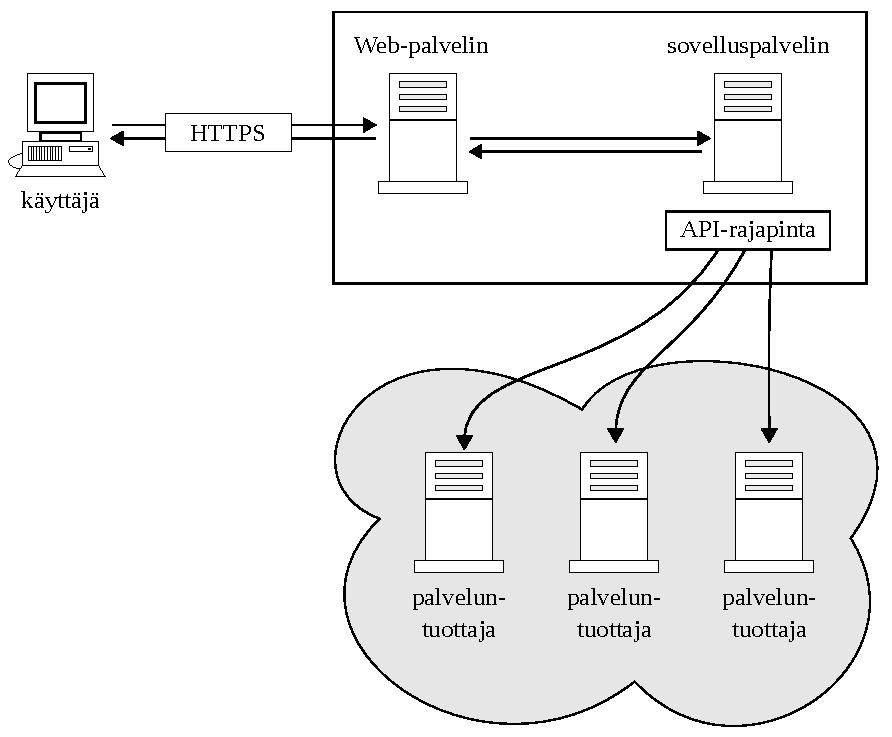
\includegraphics[width=12cm]{pics/soa_arkkitehtuuri.pdf}
\caption{Palvelukeskeinen arkkitehtuuri.}
\label{soa}
\end{figure}

\newpage

\section{Web-palveluihin kohdistuvia hyökkäyksiä}

Internetin kehittyessä myös Web-palveluihin kohdistuvat hyökkäykset ovat saaneet
uusia ilmenemismuotoja. Aikaisemmin ``Web-hakkeroinnin'' nimellä kutsuttiin
hyökkäyksiä, jotka kohdistuivat palveluita tarjoaviin alustoihin kuten Apache ja 
Microsoft IIS. Nämä hyökkäykset perustuivat tunnettujen haavoittuvaisuuksien
hyödyntämiseen, ja oikeille työkaluilla varustautunut hyökkääjä pystyi kaatamaan haavoittuvan
palvelun muutamassa minuutissa. Esimerkiksi tunnetuimpien Internet-matojen Code Redin ja Nimdan toiminta
perustui Microsoft IIS:sä olevan haavoittuvuuden hyödyntämiseen \cite{Hacking}. 

Tämänlaiset hyökkäykset ovat kuitenkin menettäneet suurimman tehonsa, koska tehdyistä virheistä on opittu. Löydettyihin 
haavoittuvaisuuksiin reagoidaan entistä nopeammin, yhä useampi alusta on konfiguroitu oikein ja saatavilla on työkaluja, joiden
avulla pystytään nopeasti ja helposti havaitsemaan yleisimmät tietoturvariskit \cite{Hacking}. Näistä seikoista johtuen
hyökkääjät ovat alkaneet kiinnittämään entistä enemmän huomiota itse alustalla pyöritettäviin palveluihin pyrkien 
murtautumaan järjestelmiin näiden kautta. Dynaamisten Web-teknologioiden myötä tämän tyyppiset hyökkäykset ovat saaneet
enemmän huomiota, sillä se tarjoaa hyökkääjille entistä monipuolisemman hyökkäyspinnan. Tietoturvan 
kannalta onkin tärkeää, että kumpaankin hyökkäystapaan kiinnitetään huomiota.

\subsection{SQL-injektio}

Virheelliseen syöttötietoon perustuvat hyökkäykset ovat jo pidemmän aikaa vaivanneet Web-pohjaisia sovelluksia.
Dynaamisten Web-sovellusten myötä hyökkäykset ovat entisestään yleistyneet, sillä monimutkaisten sovellusten takana käytetään entistä
enemmän erilaisia tietokantapohjaisia ratkaisuja kuten MySQL. Nämä hyökkäykset hyödyntävät sitä seikkaa, että suurin osa
sovelluksista ei tee selkeää eroa käyttäjän antaman syötteen ja ohjelmalle annettavien käskyjen välillä. Tämä mahdollistaa
sen, että hyökkääjä pystyy piilottamaan annettuun hakuun ohjelmatason käskyjä, jotka muokkaavat sovelluksen toimintaa
hyökkääjän haluamaan suuntaan \cite{WEB2}. Tavanomaisilla
menetelmillä, kuten palomuureilla, tällaisen hyökkäysten tunnistaminen on hankalaa, sillä
monien organisaatioiden tietoturvasta vastaavat palomuurit toimivat OSI-mallin
kolmannella, neljännellä ja viidennellä kerroksella. Tämän vuoksi
niiltä jäävät huomaamatta ylimmän kerroksen eli ohjelmistokerroksen
kautta tulevat hyökkäykset. Tämän lisäksi useimmat palomuurit eivät
ymmärrä sovellusprotokollien,
kuten HTTP:n, tarkkaa sisältöä \cite{SQLSS}.    

Onnistunut injektiohyökkäys koostuu kolmesta erillisestä vaiheesta. Ensimmäisessä vaiheessa hyökkääjän tulee tunnistaa 
Web-sovelluksessa käytetyt teknologiat. Tämä onnistuu muun muassa tulkitsemalla sivujen antamia virheilmoituksia, tutkimalla 
sivun lähdekoodia ja käyttämällä tätä tarkoitusta varten tehtyjä työkaluja kuten Nessusta ja Nmapia. Osaavalla hyökkääjälle tämä vaihe on melko triviaali, 
mutta hyökkäyksen kannalta tiedot ovat elintärkeitä, sillä injektiohyökkäyksen onnistuminen on täysin riippuvainen 
käytetystä alustasta.

Kun tarvittavat tiedot on saatu kerättyä, voidaan varsinaista hyökkäystä alkaa suunnittelemaan.
Tämä tapahtuu tunnistamalla ne syötteet, jotka käyttäjä pystyy sovellukselle antamaan. Tämä käsittää käytännössä kaiken sen 
tiedon, joka voidaan välittää HTTP:n GET- ja POST-pyynnöissä. Viimeisessä vaiheessa hyökkääjän tehtäväksi jää niiden syötteiden 
tunnistaminen, joita käyttämällä sovelluksen toimintaa saadaan muokattua. Tähänkin tehtävään löytyy useita valmiita työkaluja, ja
monessa tapauksessa samat toimintaperiaatteet toimivat monilla eri alustoilla \cite{WEB2}.

Structured Query Language (lyh. SQL), joka on alan vakiintunut standardi tietokantojen käsittelyyn, on käytössä lähes jokaisessa
Web-\-sovelluksessa, joka käyttää jonkinlaista tietokantaratkaisua. Sen syntaksi on sekoitus ohjelmakäskyjä ja käyttäjän antamia
syötteitä, ja huonosti määritettynä käyttäjän antama syöte voidaan tulkita virheellisesti ohjelmatason käskyksi. Tämän syötteen
hyökkääjä joutuu usein etsimään sokeasti, mutta syötteet kuten

\begin{itemize}
\item \texttt{' OR 1=1 "{-}{-}}
\item \texttt{') OR 1=1 "{-}{-}}
\end {itemize}
toimivat hyvin usein \cite{WEB2}. Virheellisestä hausta aiheutuvat virheilmoitukset antavat myös erittäin paljon
hyödyllistä tietoa hyökkääjälle \cite{SQLSS}. Koska suurin osa SQL-tietokannoista mahdollistaa useamman perättäisen syötteen 
antamisen, kunhan syntaksi pysyy oikeana, voidaan näiden avulla
katkaista ohjelman normaali toiminta. Otetaan esimerkiksi
seuraava Java-kielellä toteutettu SQL-kyselyn muodostaminen:

\begin{lstlisting}[language=java,aboveskip=0.5cm]
String query = "SELECT id FROM user WHERE " +
               "username='" + username + "' AND " +
               "password=PASSWORD('" + password + "')'';
\end{lstlisting}

\noindent Mikäli muuttujan \texttt{username} arvo on

\begin{lstlisting}[language=sql,aboveskip=0.5cm]
' OR 1=1;DROP TABLE user;-- 
\end{lstlisting}

\noindent tällöin tietokannalle ohjattava kysely on seuraava:

\begin{lstlisting}[language=java,aboveskip=0.5cm]
String query = "SELECT id FROM user WHERE " +
               "username='" + "' OR 1=1;DROP TABLE user;-- "+
               "' AND password = PASSWORD ('x')";
\end{lstlisting}

\noindent SQL-kielessä kaksi perättäistä viivaa tarkoittaa, että kaikki siitä oikealla puolella oleva on kommenttia. 
Näin ollen lopullinen SQL-haku on:

\begin{lstlisting}[language=sql,aboveskip=0.5cm]
SELECT id FROM user WHERE username='' OR 1=1;
DROP TABLE user;
\end{lstlisting}

\noindent Näin muodostettu haku on syntaktisesti täysin oikea. Kyseinen lause
poistaa tietokannassa olevan user-taulun, joka tässä tapauksessa
sisältää järjestelmään tallennetut käyttäjät \cite{WEB2}.

Vastaavanlaisia tekniikoita käyttäen hyökkääjä pystyy tekemään kaiken sen, joka pystytään esittämään SQL-kyselynä, ja johon ajettavalla
sovelluksella on riittävät oikeudet. Mielivaltaisten käskyjen antaminen, DLL-tiedostojen luominen ja ajaminen sekä tietokannan
sisällön lähettäminen jollekin toiselle Internetiin liitetylle palvelimelle ovat vain muutamia esimerkkejä toiminnoista, joita
onnistunut hyökkäys voi aiheuttaa \cite{SQLSS}.

Injektiohyökkäykset eivät rajoitu pelkästään SQL-kieleen, sillä useat eri tekniikat kuten XPath ja LDAP sisältävät vastaavanlaisia 
heikkouksia \cite{WEB2}. SQL-kieleen pohjautuvat hyökkäykset ovat kuitenkin kaikista yleisimpiä johtuen sen levinneisyydestä. SQL-kieleen
pohjautuvat ratkaisut sisältävät usein myös osan seuraavista ominaisuuksista, jotka mahdollistavat hyökkäysten tekemisen:

\begin{itemize}
\item Kommentoinnin mahdollistava merkkijono: \texttt{{-}{-}}
\item Mahdollisuus suorittaa useita hakuja yhdellä kertaa käyttäen puolipistettä
\item SQL-palvelimen antamat tarkat virheilmoitukset
\item Dynaaminen tyypitys -- kokonaisluvut käännetään mahdollisuuksien mukaan merkkijonoksi, jolloin hyökkääjän
             on helpompi arvata oikea syöte \cite{SQLSS}
\end{itemize}

Esille tulleiden asioiden valossa on selvää, että SQL-kieleen pohjautuvat haavoittuvuudet ovat todellinen uhka tietoturvalle.
Tästä johtuen on tärkeää, että sovellusten turvallisuus pyritään takaamaan kaikin mahdollisin tavoin. Täysin turvallisen sovelluksen 
suunnitteleminen on kuitenkin mahdoton tehtävä, mutta noudattamalla muutamia perusperiaatteita voidaan riskiä vähentää huomattavasti.

Verkon tietoturvaratkaisuja valittaessa ja suunniteltaessa
SQL-\-injektiohyökkäykset tulee ottaa huomioon.
Koska injektiohyökkäykset pyrkivät hyödyntämään syötteiden
virheellistä tulkintaa, voi hyväksyttävien syötteiden rajoittaminen
tuntua helpolta ratkaisulta ongelmaan. Osittain tämä ratkaisee asian,
mutta ongelmaksi muodostuu se, kuinka valita mikä syöte on
hyväksyttävä ja mikä virheellinen. Yksi keino on sallia ainoastaan
syötteet, jotka tiedetään etukäteen kelvollisiksi. Tällöin huono syöte
voidaan jättää kokonaan käsittelemättä. Tämä keino on kaikista
rajoittavin, koska tällöin syötteen jokainen merkki tarkistetaan ja
jos se ei ole sallittujen merkkien joukossa, niin koko haku
hylätään.

Toinen lähestymistapa suojaamiseen on riisua syötteestä ongelmalliset
merkit kuten merkkijonon päättävä symboli. Usein tämäkin on vaikea
toteuttaa käytännössä, koska joskus voi olla vaikeaa määritellä, mikä
haku on huono ja mikä hyvä. Yksi hyväksi todettu tapa onkin rajoittaa
tiettyjen merkkien käyttöä siten, että merkin ollessa haussa mukana
tämä muutetaan toiseen muotoon. Tämäkään ratkaisu ei ole täysin
ongelmaton, ja siksi usein vain hylätään koko syöte, jos se ei vastaa
odotettua syötettä \cite{SQLSS}.

Palvelinohjelmistoissa tulee myös ottaa huomioon muutamia asioita, joita seuraamalla voidaan huomattavasti parantaa yrityksen tietoturvaa.
Tietoturvan kannalta huolellisesti suunnitellun palvelinohjelmiston avulla voidaan myös pienentää huonosti suunnitellun sovelluksen riskiä joutua injektiohyökkäyksen kohteeksi. 
Seuraava lista ei ole millään tavalla täydellinen ratkaisu ongelmaan,
mutta se sisältää tärkeimpiä keinoja injektiohyökkäysten estämiseen ja
niiden vaikutusten minimointiin.

\begin{itemize}
\item SQL-palvelimen ajaminen pienillä käyttöoikeuksilla
\item Sallitaan tallennettujen proseduurien ajaminen ainoastaan järjestelmän ylläpitäjille
\item Linkitettyjen palvelimien yksinkertaisten tunnistusten poistaminen
\item Määrittää palomuuri siten, että ainoastaan luotetut käyttäjät saavat ottaa yhteyden SQL-palvelimeen. Usein ainoat, joiden yhteydet 
      tulee sallia, ovat ylläpitäjät ja Web-palvelut, joita tietokanta palvelee \cite{SQLSS}.
\end{itemize}

% Joel oikolukenut tähän asti.

\subsection{Cross-Site Scripting}
Nykyisin yhä useampi yritys on tietoinen verkon tarjoamista mahdollisuuksista ja sen mukana tulevista vaaroista. Yritykset ovat tämän johdosta
alkaneet panostamaan entistä enemmän tietoturvaan ja niistä harva toimii enää ilman kunnollista suojausta. Palomuurit ja hyökkäysten tunnistamiseen
ja estämiseen erikoistuneet sovellukset ovat myös kehittyneet viime vuosina niin paljon, että enää harva perinteinen hyökkäys toimii ilman
suuria muutoksia sen toteutustapaan. Tästä johtuen hyökkääjät ovat omaksuneet yhä salamyhkäisempiä murtautumistekniikoita, jotka pyrkivät kokonaan
ohittamaan perinteiset palomuurit. Web-pohjaiset sovellukset tarjoavat tähän erinomaisen alustan, ja dynaamisten Web-tekniikoiden myötä mahdollisuudet 
ovat vain entisestään kasvaneet.

Cross-Site Scripting eli XSS-hyökkäykset eivät ole millään tapaa uusi hyökkäystyyppi, ja joidenkin arvioiden mukaan kahdeksan kymmenestä sivustosta on 
niille jollakin asteella alttiina. XSS-hyökkäykset ovat myös viime vuosina keränneet suosiota hyökkääjien keskuudessa, sillä dynaamisten Web-sovellusten
myötä yhä useampi näistä käyttää erilaisia tiedonlähteitä sisällön keräämiseen. RSS-\-syötteet, widgetit, mashupit ja erilaiset JavaScript-pohjaiset komponentit 
tarjoavat kaikki hyökkääjille monta mahdollisuutta, johon iskeä. Tähän kun lisätään se, että sovelluksista monet päivittävät tietoja käyttäjän tietämättä, 
niin tilanteesta muodostuu entistä vaarallisempi \cite{WEB2b}. Tästä johtuen XSS-hyökkäykset muodostavat nyt ja tulevaisuudessa erittäin suuren riskin
tietoturvalle.

Painotuksen siirtyminen kohti Web-pohjaisia hyökkäyksiä on ollut selkeästi havaittavissa jo pidemmän aikaa. Vuonna 2007 johtava tietoturva-alan 
yritys Symantec julkisti raportin, jonka  mukaan vuoden 2007 viimeisen kuuden kuukauden aikana raportoiduista haavoittuvaisuuksista 11,253
oli sivustokohtaisia XSS tietoturva-aukkoja. Tätä lukua kun vertaa muihin löydettyihin riskeihin, joita oli 2,134, niin 
yli 80 prosenttia löydetyistä tietoturva-aukoista oli Web-pohjaisia \cite{SYM}. Vuonna 2009 julkistetussa raportissa tilanne oli lähes yhtä paha, 
sillä 63 prosenttia haavoittuvaisuuksista kohdistui Web-sovelluksiin \cite{SYM2}.

Kuten aikaisemmin on tullut esille, niin injektiohyökkäykset eivät rajoitu pelkästään tietokantasovelluksiin. Myös XSS-hyökkäykset ovat eräänlaisia 
injektiohyökkäyksiä sillä erotuksella, että hyökkääjä ei suoraan toteuta injektiota vaan uhri tekee sen itse. Tähän hyökkääjällä on useita eri 
keinoja, ja harvoin käyttäjä edes huomaa joutuneensa hyökkäyksen kohteeksi. Hyökkäyksen onnistuessa Web-sivujen käyttämä Same Origin -pe\-ri\-aa\-te 
voidaan kiertää, jolloin hyökkääjän on mahdollista ajaa kohteen selaimessa haluamaansa koodia ja skriptejä. Tämä saman alkuperän periaate on Web-selainten 
yksi tärkeimmistä suojausmenetelmistä, ja se estää muun muassa skriptien lataamisen yhdestä lähteestä hakemalla tai asettamalla määrityksiä toisesta lähteestä \cite{WEB2}.

\begin{figure}[htp]
\centering
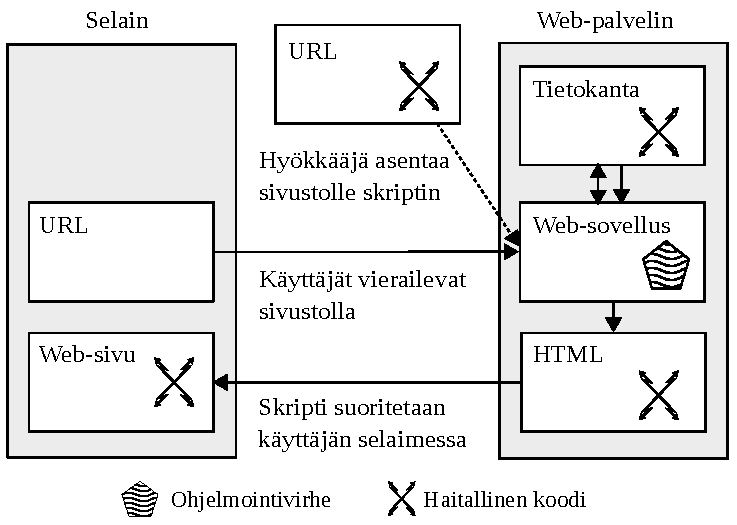
\includegraphics[width=12cm]{pics/tallennettu.pdf}
\caption{Palvelimelle tallennettu XSS-hyökkäys.}
\label{tallennettu}
\end{figure}

XSS-hyökkäykset jaetaan heijastettuihin ja tallennettuihin hyökkäyksiin sen mukaan, kuinka hyökkäys on toteutettu. Tallennetussa hyökkäyksessä haavoittuvalle 
Web-sivustolle asennetaan pysyvästi vihamielinen skripti, joka ajetaan
sivun vierailun yhteydessä (kuva \ref{tallennettu}). Tällaiset skriptit ovat yleensä kirjoitettu JavaScriptillä
ja ne voidaan tallentaa esimerkiksi Web-palvelimen tietokantaan, kommenttikenttiin tai foorumin viesteihin. Koska selain luottaa siihen, 
että sivuston sisältö on luotettavasta lähteestä, pystyy hyökkääjä tämän jälkeen lukemaan ja muokkaamaan selaimen arkaluontoista sisältöä. Evästeet, jotka ovat Web-sovellusten 
toiminnan kannalta erittäin tärkeitä, ovat ensimmäisiä kohteita joihin yritetään yleensä päästä käsiksi, sillä ne ylläpitävät yhteyksien tiloja eri 
sivustoille ja oikean käyttäjän tunnistamiseen tarvittavia tietoja \cite{WEB2b}. Näitä kaappaamalla hyökkääjä pystyy esiintymään verkossa toisena käyttäjänä 
ja väärinkäyttämään palveluita kuten verkkopankkia tai webmailia. 

Heijastettu hyökkäys (kuva \ref{heijastettu}) eroaa tallennetusta hyökkäyksestä siten, että haitallista skriptiä ei tallenneta minnekään pystyvästä. Hyökkäyksen kohteeksi käyttäjä joutuu, kun 
hänet huijataan esimerkiksi painamaan vihamielistä linkkiä, joka tekee käyttäjän puolesta kyselyn haavoittuvalle sivustolle. Haavoittuva sivusto heijastaa kyselyn tuloksen 
takaisin käyttäjälle esimerkiksi virheviestin tai hakutuloksen muodossa, ja näin toimitettu koodi suoritetaan käyttäjän selaimessa, koska se tulee selaimen luottamalta
osapuolelta  \cite{WEB2}.

\begin{figure}[htp]
\centering
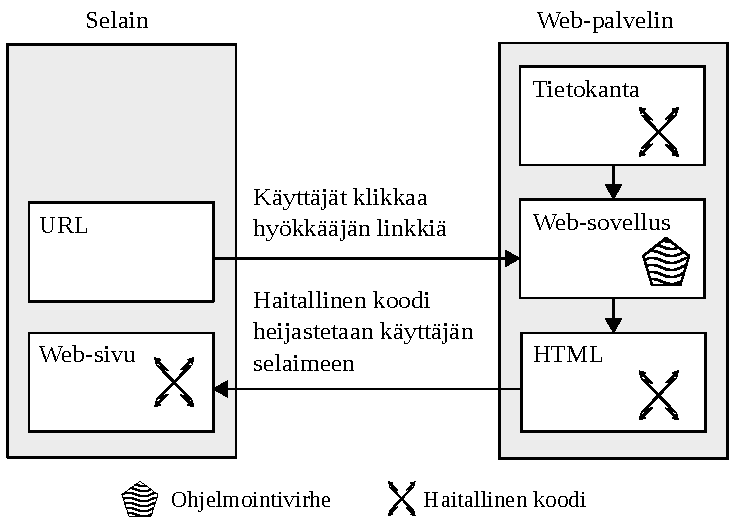
\includegraphics[width=12cm]{pics/heijastettu.pdf}
\caption{Palvelimelta heijastettu XSS-hyökkäys.}
\label{heijastettu}
\end{figure}

Hyökkääjän mahdollisuudet eivät rajoitu pelkästään evästeiden varastamiseen. Onnistuneen XSS-hyökkäyksen jälkeen hyökkääjä voi esimerkiksi ohjata
käyttäjän osoitteeseen, joka jäljittelee haluttua sivustoa. Käyttäjän yrittäessä kirjautua tähän palveluun, saa hyökkääjä selville käyttäjän tunnuksen ja
salasanan. XSS-hyökkäykset tarjoavatkin erinomaisen mahdollisuuden toteuttaa \textit{phishing} eli tiedon kalasteluhyökkäyksiä. XSS-\-madot ovat
myös viime aikoina yleistyneet, sillä yhä useampi palvelu on niille haavoittuvainen. Esimerkiksi Webmail-sovelluksia varten kirjoitetut madot 
käyttävät hyödyksi sitä seikkaa, että hyökkääjä pääsee käsiksi uhrin kontaktilistaan. Tällainen mato pyrkii leviämään lähettämällä 
kontaktilistalla oleviin osoitteisiin sähköpostia, ja koska viesti tulee luotettavasta osoitteesta, ei käyttäjät osaa usein varoa viestissä
olevaa linkkiä. Hyökkääjä vielä usein muokkaa linkistä sen näköisen, että vastaanottaja ei osaa epäillä linkin aitoutta \cite{WEB2}. 
XSS-madot leviävätkin usein todella nopeasti, ja ne kuljettavat usein myös muita hyökkäyksiä mukanaan. Tästä hyvänä esimerkkinä
Sammy-madoksi nimetty XSS-hyökkäys, joka vuonna 2005 iski MySpace-sivustolle, joka on yksi tunnetuimmista sosiaaliseen verkostoistumiseen
erikoistuneista sivustoista. Käyttäen sivustossa olevaa heikkoutta hyväkseen mato saastutti käyttäjien sivuja, ja jonkun vieraillessa 
saastuneella sivulla, saastui myös hänen oma MySpace sivunsa. 24 tunnissa mato oli saastuttanut yli miljoona sivua, ja tilanteen korjaamiseksi
MySpace joutui sulkemaan väliaikaisesti sivustonsa. Hyökkäyksen vahingot eivät rajoittuneet tähän, vaan seuraavina viikkoina useista tunnetuista sivustoista
kuten Googlesta ja Yahoosta löytyi vastaavanlaisia tietoturva-aukkoja \cite{WEB2b}.

Tärkein asia XSS-hyökkäysten estämiseksi on olla tarkkana sen suhteen, kuinka käyttäjien tarjoama sisältö välitetään toisille käyttäjille.
Tärkeää on myös muokata käyttäjän antama syöte aina sellaiseen muotoon, että kun palvelin lähettää esimerkiksi virhesanomassa käyttäjän antaman syötteen
takaisin, niin ei tätä voida käyttää sellaisenaan hyökkäyksen toteuttamiseen. Tiettyjen merkkien poistamisella voidaan hyökkäyksiä vähentää,
mutta usein merkkien kuten heittomerkin (') poistaminen ei tule kyseeseen. Suunnittelijoiden avuksi on myös olemassa suuri määrä sovelluksia, jotka
etsivät sivustoilla olevia heikkouksia \cite{WEB2}. Tämän suhteen tulee kuitenkin muistaa, että myös hyökkääjillä on käytettävissä samat sovellukset, joten 
näillä löydetyt tietoturvariskit tulisi korjata mahdollisimman nopeasti. Symantecin raportin mukaan näin kuitenkin tapahtuu todella harvoin, sillä 6,961 
sivustosta vain 473 oli korjattu raportin kirjoittamisen aikana, ja tähänkin oli mennyt keskimäärin 52 päivää \cite{SYM}. XSS-haavoittuvista sivuista
kirjaa pitävän sivuston mukaan tilanne ei ole nykyisin yhtään sen parempi, sillä suurin osa löydetyistä sivuista on edelleen korjaamatta \cite{XSS}.
Näyttääkin siltä, että yritykset ymmärtävät asian vakavuuden vasta sitten, kun sivusto on joutunut hyökkäyksen kohteeksi.

\subsection{Cross-Site Request Forgery}

Dynaamisten Web-sovellusten yksi keskeisimmistä selaimessa toimivista ratkaisuista on Document Object Modeliksi (lyh. DOM) nimetty rakenne, joka on vastuussa siitä,
kuinka Web-sivun sisältöä käsitellään, ja kuinka eri objektit kommunikoivat keskenään. Tämä rakenne vastaa siitä, että ainoastaan saman domainin 
sisäinen kommunikointi ja sisällön muokkaaminen on sallittu. Tämä ratkaisu poistaa sen mahdollisuuden, että Web-sivun DOM:ia voitaisiin muokata toisen
domainin kautta. Tämä vastaa saman alkuperän periaatetta, jolla pyritään estämään Web-sivuihin ja käyttäjiin kohdistuvia vihamielisiä toimia.
Webin muuttuessa entistä interaktiivisemmaksi, ovat sivustot kuitenkin alkaneet sallia yhä enemmän domainien välistä kommunikointia. Tällaisia 
toimia ovat esimerkiksi hyperlinkkien käyttäminen sisällön näyttämisessä, kuvien ja objektien lataaminen sekä toisessa domainissa olevien 
JavaScriptien ajaminen. Nämä ja monet muut toimet ovat mahdollistaneet entistä monipuolisempien Web-palveluiden suunnittelun, mutta huonosti toteutettuna 
ne jättävät palvelut hyvin haavoittuviksi. Tämä johtuu siitä, että käyttäjän tarkoituksella tekemiä toimia ei pystytä erottamaan niistä toimista, jotka tehdään 
automaattisesti käyttäjän vieraillessa sivustolla \cite{WEB2}.

XSS-hyökkäysten tapaan myös Cross-Site Request Forgery (lyh. CSRF) hyökkäykset ovat jo pidemmän aikaan olleet olemassa, mutta vasta viime vuosina ne
ovat yleistyneet. Ero näiden kahden hyökkäyksen välillä on siinä, että missä XSS skripti suoritetaan käyttäjän selaimessa, niin CSRF hyökkäyksessä käytetyt
käskyt ja skriptit kohdistetaan Web-palveluihin, joiden kanssa selaimella on luottamussuhde. CSRF toteutetaan siten, että hyökkääjä asettaa jollekin sivulle
vihamielisiä tageja, joiden avulla voidaan luoda haitallisia HTTP-pyyntöjä. Nämä pyynnöt kohdistetaan johonkin toiseen domainiin ja ne ajetaan käyttäjän 
vieraillessa kyseisellä sivustolla. Jos käyttäjän selaimella on sitten esimerkiksi tähän domainiin liittyvä eväste voimassa, voidaan HTTP-pyynnöillä pyytää muun muassa
salasanan vaihtoa tai sähköpostin lähettämistä käyttäjän nimissä \cite{WEB2b}. Hyökkääjä pystyy tällä tavoin myös ottamaan yhteyttä sellaisiin koneisiin ja palveluihin,
joihin hänellä ei muuten olisi oikeuksia johtuen esimerkiksi palomuurista tai IP-osoitteiden suodatuksesta \cite{CSRF}.

CSRF hyökkäysten teho perustuu siihen, että monet sivustot ja palvelut
käyttävät evästeitä melko huolimattomasti. Evästeitä käytetään
käyttäjän yksilöimiseen ja tunnistamiseen, joten riittää, että hyökkääjä pääsee niihin käsiksi tavalla tai toisella. Useat sivustot myös sallivat käyttäjien pysyvän kirjautuneena sisällä
jopa useita viikkoja, jolloin sama eväste on pitkään käytössä. Monien sovellusten ja pyyntöjen rakenne on myös hyvin ennalta arvattavissa, jolloin hyökkääjän
on helpompi arvata käskyjen ja parametrien oikea muoto \cite{WEB2}.

CSRF hyökkäykset eivät rajoitu pelkästään perinteisiin Web-tekniikoihin, sillä suurin osa dynaamisista teknologioista ovat sille jollakin 
tavalla alttiina. Erityisesti AJAX ja JavaScript ovat tuoneet mukanaan suuren joukon uusia haasteita, jotka suunnittelijoiden tulee ottaa huomioon uusien
sovelluksien suunnittelussa \cite{WEB2b}. Täydellinen suojautuminen CSRF-\-hyökkäyksiltä vaatii syvällistä osaamista käytetyistä tekniikoista, ja 
tietämystä eri komponenttien välisistä toiminnoista. Puutteellisista
toteutuksista johtuen monet sivustoista ja palveluista ovat haavoittuvaisia
CSRF-hyökkäyksille. Tästä tunnettuna esimerkkinä sähköpostisivusto Gmail, josta löytyi vuonna 2007 CSRF-hyökkäyksen mahdollistava heikkous. Tämän avulla
hyökkääjän oli mahdollista luoda Gmailiin sellainen suodatus, joka ohjasi tulevat postit toiseen osoitteeseen \cite{CSRF}. 

CSRF-hyökkäyksiltä suojautumiseen on käytössä kolme hyvin yleistä tekniikkaa. Näistä käytetyin on sisällyttää jokaiseen palvelinpuolen dataa muokkaavaan
GET/POST pyyntöön mukaan salattu tokeni, jonka avulla jokainen pyyntö voidaan yksilöidä ja tunnistaa kuuluvan oikeaan istuntoon. Tämä salattu tokeni tekee
käyttäjän syötteestä arvaamattoman muotoisen, jonka johdosta CSRF-hyökkäyksen toteuttaminen on hyvin vaikeaa \cite{WEB2}. Yksinkertaisin suojausmenetelmä on 
taas tunnistaa HTTP-kyselyn Referer-otsake, ja hyväksyä vain sellaiset pyynnöt, jotka tulevat luotettavista lähteistä. Kolmas menetelmä on tehdä kustomoituja
otsakkeita käyttäen XMLHttpRequestia, jonka käyttö on lisääntynyt AJAXin yleistyessä. Kustomoitujen otsakkeiden oikeellisuus sitten varmistetaan, ennen kuin
pyynnöt käsitellään palvelinpuolella \cite{CSRF}.

Nämä kolme esitettyä tapaa ovat yleisimmin käytössä, mutta nekin sisältävät joukon heikkouksia. Salatun tokenin ongelma on siinä, että kyseisestä tekniikasta ei 
ole olemassa yleisesti sovittua toteutustapaa. Tämä aiheuttaa sen, että useat ratkaisut ovat tavalla tai toisella puutteellisia. Referer-otsakkeiden suodatuksen 
ongelma on siinä kuinka käsitellä pyyntöjä, joista puuttuu Referer-otsake. Otsakkeen piilottaminen ei ole vaikea tehtävä, joten palvelin saattaa joutua 
päättämään vajailla tiedoilla päästääkö pyyntö läpi vaiko suodattaa se pois. XMLHttpRequestin käyttöä taas rajoittaa sen tuomat lisävaatimukset toteutukselle,
joka rajoittaa tiettyjen palveluiden käyttöä \cite{CSRF}. 

Näiden ja monien muiden syiden takia tutkimustyö CSRF-hyökkäysten parissa on kasvattanut suosiotaan. Yhdessä tutkimuksessa ehdotettiin erillisen Origin
otsakkeen lisäämistä pyyntöön, joka korjaisi Referer-kentän heikkoudet \cite{CSRF}. Toisessa tutkimuksessa taas pyrittiin kasvattamaan Web-selaimen turvallisuutta
lisäämällä selaimeen mekanismi, joka pyrki arvioimaan vastasiko tehdyt pyynnöt käyttäjän toimia \cite{CSRFb}. Näistä kahdesta erilaisesta ratkaisusta on nähtävissä se,
että tutkimuskenttä CSRF-hyökkäysten ympärillä on hyvin alkuvaiheessa, ja vastuu riittävän suojauksen hoitamisesta jää vielä tällä hetkellä 
sovelluksen kehittäjälle ja ylläpitäjälle.

\section{Web-palveluiden tietoturvan parantaminen}

Web-palveluiden ja verkon tietoturvasta vastaaminen on tarkkuutta ja aikaa vaativaa työtä, joka edellyttää omien tietojen jatkuvaa päivittämistä sekä ja liikenteen ja palveluiden
seuraamista. Jo pelkästään yleisimpien tietoturvariskien tunnistaminen ja korjaaminen osoittautuu usein käsin tehtynä ylivoimaiseksi tehtäväksi verkkojen ja palveluiden
muuttuessa entistä monimutkaisemmiksi. Työn helpottamiseksi on saatavilla useita työkaluja, joiden avulla sekä kehittäjät että ylläpitäjät voivat
etsiä sovelluksista ja verkoista tunnetuimpia tietoturva-aukkoja. Osa näistä pohjautuu vapaaseen lähdekoodiin, mutta tarjolla on myös kaupallisia sovelluksia, jotka ainakin 
paperilla lupaavat parempia ominaisuuksia. Näiden lisäksi palvelinpuolella on tarjolla erilaisia lisäosia, jotka lisäävät Web-palveluiden tietoturvaa. 
Mikään sovellus ei tietenkään voi löytää jokaista tietoturvariskiä, joten pelkästään näiden varaan ei voida tietoturvaa rakentaa. Näiden avulla 
saadaan kuitenkin hyvä yleiskuva siitä, minkälaisille heikkouksille sovellus on mahdollisesti alttiina, ja kuinka verkon turvallisuutta voidaan parantaa. Koska samat 
sovellukset on myös hyökkääjien käytössä, niin ainakin aukot, jotka löytyvät yleisimmin käytössä olevilla työkaluilla, tulisi korjata mahdollisimman nopeasti. 

Web Application Security Consortium (lyh. WASC) on vuonna 2004 perustettu avoin kansainvälinen ryhmittymä, joka koostuu tietoturva-alan asiantuntijoista sekä eri 
yritysmaailman tahoista, joiden tavoitteena on tuottaa vapaaseen käyttöön best practice -malleja ja standardeja turvallisesta Internetistä. Se julkaisee
erilaisia artikkeleita, esitysmateriaaleja ja tietoturvalinjauksia, joita käytetään hyvin laajasti ohjenuorina yritysmaailmassa sekä tuotekehityksessä \cite{WASC}.
WASC:n tämän hetkisiin projekteihin kuuluvat Web-sovellusten turvallisuuden tutkimiseen käytettävien ohjelmistojen arviointikriteerien laatiminen sekä tilastointi
Web-sovellusten turvallisuudesta. Viimeisimmän WASC:n tekemän raportin mukaan tutkituista sivustoista, joita oli yhteensä 12186 kappaletta ja joista löytyi 97554 
eri asteista tietoturvariskiä, 13 prosenttia pystyttiin murtamaan täysin automaattisesti, ja noin 49 prosenttia Web-sovelluksista sisälsi helposti havaittavia vakavia 
tietoturvariskejä. Tämä luku kasvoi jopa 96 prosenttiin, kun sivuston tutki tietoturva-alan asiantuntija. Huomattavaa oli myös se, että sivustoista 99 prosenttia
ei noudattanut alan standardeja, ja ylläpidon aiheuttamat haavoittuvaisuudet olivat 20 prosenttia yleisempiä kuin sovelluskehittäjien tekemät. Tutkimus myös 
osoitti sen, että XSS-hyökkäykset olivat SQL-injektiohyökkäysten ohella kaikista yleisimpiä \cite{WASCb}. Tämän tiedon valossa onkin tärkeää, että sekä sovelluksen
kehittäjä että ylläpitäjä ovat ajan tasalla palvelun nykyisestä tilasta. 

\subsection{Tietoturvastrategia}

Tietoturvan kannalta on tärkeää, että verkon ylläpitäjä tietää tarkoin
kuinka verkko toimii ja sen valvonnassa hyödynnetään verkon
analysointityökaluja. Näiden avulla verkon heikot kohdat pystytään
tunnistamaan ja vahvistamaan. Käytössä tulee olla myös jonkinlainen
suojausjärjestelmä, joka kirjaa ylös riittävän pitkältä ajalta ylös
verkkoon tulevan ja lähtevän liikenteen, sillä esimerkiksi hajautettu
palvelunestohyökkäys ei aina kaada koko verkkoa. Tällöin on tärkeää,
että tapahtunut pystytään tarkasti analysoimaan ja löydetyt heikkoudet
paikattua parhaalla mahdollisella tavalla \cite{DDOS}.

Kun hyökkäys on meneillään, tulee käytetty hyökkäystapa tunnistaa mahdollisimman
nopeasti. Useimmat hyökkäykset noudattavat tiettyä kaavaa ja näiden
tunnistamiseen on olemassa useita valmiita työkaluja. Tämä on tärkeää, koska
tunnistamisen jälkeen voidaan rajata, mistä hyökkäys on peräisin ja tehdä
tarvittavat toimenpiteet hyökkäyksen torjumiseksi. Useimmissa tapauksissa
tämä tarkoittaa yhteistyötä palveluntarjoajan ja viranomaisten kanssa.
Viranomaisten mukaan tuominen on muutenkin tärkeää, koska vain tätä kautta
voidaan käytettyä hyökkäysverkostoa lähteä tunnistamaan ja toivottavasti myös
hajottamaan \cite{DDOS}.

Jotta nopea reagoiminen olisi mahdollista, tulee organisaatiolla olla
toimintasuunnitelma hyökkäyksen varalta. Ensimmäinen vaihtoehto lienee aina
haitallisen liikenteen estäminen, mutta tätä varten tulee olla tehtynä tarkat
prosessit kuinka toimitaan hyökkäyksen alettua. Tärkeää on sopia mitä
dokumentoidaan ja kuinka asioista raportoidaan oikeille tahoille. Hyökkäyksen
jälkeinen analyysi on myös riippuvainen sovituista käytännöistä. Tämä analyysi
on erittäin tärkeää, sillä vain sitä kautta toimintasuunnitelmia voidaan
kehittää oikeaan suuntaan \cite{DDOS}.

\subsection{Web-alustojen tietoturva}

Aikaisemmin esitetyt seikat eivät tarkoita sitä, että Web-palveluita pyörittävät alustat olisivat
turvassa hyökkäyksiltä. Onnistuneet hyökkäykset ovat edelleen yhtä tuhoisa, jos niihin ei varauduta ennalta.
Erilaiset hyökkäykset pyrkivät yleensä hyödyntämään seuraavissa kategorioissa olevia heikkouksia

\begin{itemize}
\item Valmiit esimerkkitiedostot
\item Lähdekoodin paljastuminen
\item Kanonisointi
\item Palvelimiin asennetut lisäosat
\item Syötteen tarkistaminen \cite{Hacking}.
\end{itemize}
Kanonisoinnilla tarkoitetaan sääntöjen mukaisen syötteen väärinkäyttöä. Hyökkäys pohjautuu siihen,
että useimpia palveluita ja resursseja voidaan kutsua monin eri
tavoin. Esimerkiksi tiedostoon \texttt{C:\textbackslash text.txt}
voidaan suhteellisesti viitatata syntaksilla \texttt{..\textbackslash text.txt}. Sovellukset, jotka tekevät tietoturvapäätökset käyttäen hyödyksi resurssinimeä,
voidaan helposti huijata suorittamaan odottamattomia toimintoja \cite{Hacking}.

Listatuilta asioilta suojautuminen on melko yksinkertaista, kunhan noudattaa muutamia perussääntöjä. Ensinnäkin tuotannossa 
olevilla palvelimilla ei tulisi koskaan olla asennettuna tai käytettynä tiedostoja, joiden turvallisuudesta ei ole
takeita. Näihin tiedostoihin lukeutuvat muun muassa paketeissa mukana tulevat esimerkkitiedostot ja palvelimelle asennettavat 
lisäosat, joiden alkuperästä ei ole varmuutta. Toisekseen on tärkeä varmistaa, että käytettyihin sovelluksiin
on asennettu viimeisimmät päivitykset, sillä ne yleensä korjaavat tunnetut heikkoudet \cite{Hacking}. Jo pelkästään näillä 
toimilla pystytään suurimmaksi osaksi estämään sellaiset hyökkäykset, jotka kohdistuvat itse käytettyyn palvelinalustaan.
Spoofing- ja palvelunestohyökkäyksiltä nämä eivät suojaa, ja tästä syystä resursseihin kohdistuville hyökkäyksille
tulee olla erilliset suojausmenetelmät.

\subsection{Snort}

Tietoturvahyökkäysten siirtyessä hiljalleen verkkokerrokselta sovelluskerrokselle, eivät perinteiset palomuurit pysty enää yksin takaamaan riittävää tietoturvatasoa. Tästä syystä näiden
rinnalle on kehitetty erilaisia tietoturvasovelluksia, joista yleisimpiä ovat IDS- ja IPS-järjestelmät. Näistä tunnetuin ja käytetyin on vapaaseen lähdekoodiin perustuva Snort \cite{Snort}, jolla 
on rekisteröityneitä käyttäjiä lähes kolmesataatuhatta. Snortia on ladattua miljoonia kertoja ja sitä käyttävät niin yksityiset tahot kuin myös suuret yritykset ja eri valtioiden virastot. Suuren
levinneisyyden takia Snortia kutsutaan usein IPS-järjestelmien alan de facto sovellukseksi.

Snort on pohjimmiltaan sääntöpohjainen IDS-järjestelmä eli se pyrkii tunnistamaan hyökkäykset vertaamalla tulevaa liikennettä ennalta kirjoitettuihin sääntöihin. Tämä tunnistaminen toteutetaan
verkkotasolla tutkimalla jokainen tuleva paketti. Suuren käyttäjämääränsä ansiosta Snortin käyttämät säännöstöt ovat hyvin kattavat, ja yleisimpiin hyökkäyksiin kirjoitetaan
nopeasti uudet säännöt. Snortiin on myös saatavilla useita lisäosia, joiden avulla on esimerkiksi mahdollista estää tietystä osoitteesta tuleva liikenne sekä tallentaa ja analysoida haluttu liikenne. 

Koska Snortin lähdekoodi on vapaasti saatavilla, on tämän pohjalta kirjoitettu uusia järjestelmiä, joiden avulla pystytään muun muassa luomaan uusia sääntöjä automaattisesti verkkoliikenteestä 
\cite{SnortRule} ja tutkimaan verkkoliikennettä erillisinä tapahtumaketjuina \cite{SnortSet}. Näitä järjestelmiä kutsutaan usein hybridi IDS-järjestelmiksi, ja tällaisia löytyy useita erilaisia. 
Näitä ja muita sääntöpohjaisia IDS-järjestelmiä vaivaa kuitenkin sama ongelma, eli ne ovat täysin riippuvaisia oikeanlaisesta säännöstöstä. Jos tehtyyn hyökkäykseen ei löydy suoraan sääntöä, 
ei järjestelmä pysty tätä havaitsemaan. Hyökkäysten muuttuessa yhä monimutkaisemmiksi, on tästä muodostunut todellinen ongelma sääntöpohjaisille järjestelmille. Toinen ongelma IDS-järjestelmillä
on niiden tapa luoda isoilla datamäärillä suhteellisen paljon virheellisiä tunnistuksia. Näistä rajoituksista huolimatta sääntöpohjaiset IDS-järjestelmät ovat tällä hetkellä suosituin tapa
suojautua verkkohyökkäyksiltä. 

\subsection{Nikto}

Nikto \cite{Nikto} on avoimeen lähdekoodiin perustuva ilmainen Web-skanneri, joka etsii Web-sivustoilta haavoittuvia CGI-skriptejä ja tiedostoja. Sen tietokanta käsittää
yli 3500 tunnettua haavoittuvuutta sekä yli 900 eri Web-alustoihin liittyvää heikkoutta. Nikto on koodattu käyttäen Perliä ja se pyrkii skannaamaan palvelimen 
mahdollisimman lyhyessä ajassa. Tästä syystä sen aiheuttama liikenne on helppo havaita lokeista. Tämän kiertämiseksi Niktoon on lisätty mahdollisuus käyttää Whiskerin
tarjoamaa libWhisker kirjastoa, joka pyrkii ohittamaan käytössä olevat suojausjärjestelmät. Nikto on erittäin tehokas ja käytetty työkalu perusturvallisuuden 
varmistamiseen, ja vuonna 2006 tehdyssä tutkimuksessa se valittiin parhaimmaksi Web--haavoittuvaisuuksia skannaavaksi sovellukseksi \cite{INS}.
Nikton tietokantoja päivitetään hyvin satunnaisesti, joten nykyisellään se ei tunnista kaikista uusimpia hyökkäyksiä. Tästä huolimatta se on erittäin tehokas työkalu 
tietoturvan parantamiseen.

\subsection{Nessus}

Nessus \cite{Nessus} oli alunperin vapaaseen lähdekoodiin perustuva ilmainen tietoturvaskanneri, joka muuttui maksulliseksi vuonna 2008. 1200 dollarin vuosimaksua vastaan
saa kuitenkin yhden parhaimmista UNIX- ja Windows-alustoilla toimivista tietoturvaskannereista \cite{NST}. Se sisältää yli 20000 erillistä lisäosaa,
ja sen avulla on mahdollista suorittaa muun muassa reaaliaikaista liikenteen tarkkailua, konfigurointitiedostojen auditointia sekä eri verkko-osien skannausta. Maksullisuuden 
ansiosta Nessus pystytään pitämään ajan tasalla uusimmista hyökkäyksistä ja se soveltuukin erinomaisesti suurten ja monimutkaisten verkkojen turvaamiseen\cite{Nessus}. 

\subsection{Paros Proxy}

Paros Proxy \cite{Paros} on Javalla kirjoitettu HTTP-välityspalvelin, jonka avulla voidaan arvioida Web-sovelluksen turvallisuutta. Se mahdollistaa kokonaisten sivustojen indeksoimisen,
jonka lisäksi sen avulla on mahdollista tallentaa ja muokata reaaliajassa käyttäjän ja palvelimen välistä HTTP- ja HTTPS-liikennettä mukaan lukien evästeitä. Sen mukana tulee
myös skanneri yleisimpien Web-haavoittuvuuksien tunnistamiseen. Paros pohjautuu vapaaseen lähdekoodiin ja se on hyvin käytetty työväline tietoturva-\-ammattilaisten
parissa, jotka etsivät sivustoilta haavoittuvuuksia.

\subsection{ModSecurity}

Koska nykyisistä hyökkäyksistä yhä useampi kohdistuu verkon laitteiden ja resurssien sijasta Web-palveluihin ja -sovelluksiin \cite{WASCb} \cite{SYM}, eivät perinteiset
tietoturvaratkaisut pysty enää tarjoamaan riittävää tietoturvatasoa. Tästä syystä sovelluskehittäjät ja ylläpitäjät ovat joutuneet etsimään uusia ja entistä tehokkaampia 
tapoja hyökkäysten tunnistamiseen ja torjumiseen. Yksi mahdollinen ratkaisu on lisätä erillinen, Web-sovelluksia varten suunniteltu palomuuri, käyttäjän ja palvelimen 
välille, jolloin palvelulle tulevat pyynnöt kulkevat tämän palomuurin kautta. Tällä tavoin saapuva liikenne voidaan tutkia ja suodattaa käyttäen haluttuja määrityksiä. 

ModSecurity \cite{Mod} on Apachelle suunniteltu, vapaaseen lähdekoodiin pohjautuva palomuuri, joka tarjoaa kattavan suojan Web-palveluihin kohdistuvilta hyökkäyksiltä. 
Se mahdollistaa HTTP-liikenteen monitoroinnin ja reaaliaikaisen liikenteen analyysin vaatien korkeintaan hyvin pieniä muutoksia jo olemassa olevaan arkkitehtuuriin.
ModSecuritystä on saatavilla kaupallisia lisenssejä sekä tukipalveluita, mutta sovelluksen käyttämät perussäännöt ovat ilmaiseksi ladattavissa, tosin näitä
ei ole hetkeen päivitetty. ModSecurityn käyttämä säännöstä mahdollistaa kuitenkin uusien sääntöjen kirjoittamisen omien tarpeiden mukaan, joten käytetyt säännöt voidaan räätälöidä 
tilannekohtaisesti \cite{Mod}. 

ModSecurityn parhaimpiin ominaisuuksiin kuuluu mahdollisuus ylläpitää täydellistä lokia koko HTTP-tapahtuman ajalta, jolloin sekä pyynnöt että vastaukset pystytään analysoimaan.
Tämän ansiosta myös tulevien POST-pyyntöjen sisältö ja rakenne voidaan
tutkia. Nämä pyynnöt jäävät normaalisti tallentamatta lokiin, jolloin
hyökkääjän kiinnijäämisen riski on pienempi. Suurin osa hyökkäyksistä toteutetaankin 
nykyisin POST-metodia käyttämällä. Se, mitä halutaan lokittaa, voidaan myös tarkkaan määrittää. Salattu ja pakattu liikenne ei myöskään aiheuta ongelmia, sillä lokitus tapahtuu sillä tasolla,
jossa pyynnöt ovat valmiiksi puretussa muodossa \cite{Mod}.

Liikenteen kirjaamisen ohella ModSecurity voidaan määritellä estämään tulevia hyökkäyksiä, jonka lisäksi sen avulla pystytään nopeasti paikkaamaan löydetyt haavoittuvaisuudet. 
Ensinnäkin kaikki tulevat paketit voidaan pisteyttää halutulla tavalla, ja tietyn pisterajan ylittäneet paketit voidaan esimerkiksi pudottaa pois. Toinen mahdollisuus on sallia vain 
tietynlaiset pyynnöt. ModSecurityn käyttämä säännöstökieli mahdollistaa myös palveluiden nopean suojaamisen uusilta hyökkäyksiltä ilman, että palvelun omaan koodiin tarvitsee koskea.
Tämä on erityisen hyödyllistä niissä tilanteissa, joissa päivitysten tuominen tuotantoon vie aikaa. 
